\documentclass[12pt]{article}
\usepackage{amsfonts,amssymb,amsmath,epsfig}
%\documentstyle[12pt,amsfonts]{article}
%\documentstyle{article}
\usepackage{graphicx}

\setlength{\topmargin}{-.5in}
\setlength{\oddsidemargin}{0 in}
\setlength{\evensidemargin}{0 in}
\setlength{\textwidth}{6.5truein}
\setlength{\textheight}{8.5truein}
\setcounter{MaxMatrixCols}{15}
%\input ../basicmath/basicmathmac.tex
%
%\input ../adgeomcs/lamacb.tex
%\input mac-new.tex
%\input mathmac-v2.tex
%\input ../adgeomcs/mac.tex
%\input ../adgeomcs/mathmac.tex

\def\fseq#1#2{(#1_{#2})_{#2\geq 1}}
\def\fsseq#1#2#3{(#1_{#3(#2)})_{#2\geq 1}}
\def\qleq{\sqsubseteq}

%
\begin{document}
\begin{center}
\fbox{{\Large\bf Fall 2016 \hspace*{0.4cm} CIS 515}}\\
\vspace{1cm}
{\Large\bf Fundamentals of Linear Algebra and Optimization\\
Jean Gallier \\
\vspace{0.5cm}
Project 2}\\[10pt]
Due October 27, 2016\\
Frankie Leech, Chen Xiang, Reffat Manzur\\
\end{center}

\vspace{0.5cm}

\medskip

In this project, we explore properties of Haar wavelets in the context of audio signals and images. The functions that we create for this project include: {\tt haar},{\tt haar\_inv},{\tt haar\_step},\\{\tt haar\_inv\_step},{\tt haar2D},{\tt haar\_inv2D},{\tt haar2D\_n},and {\tt haar\_inv2D\_n}.
\medskip\\
(1) Graph of $plf(u)$ over the interval [0,1):\\
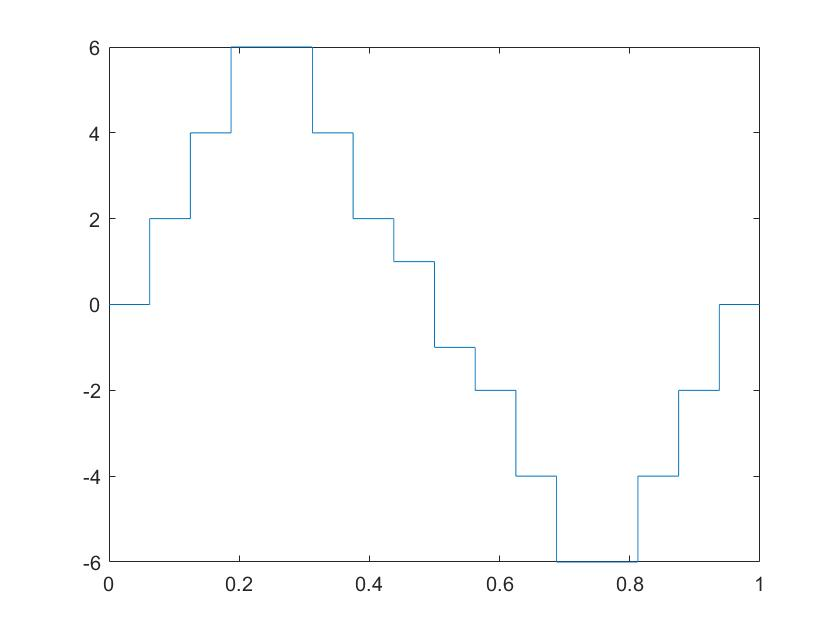
\includegraphics[scale=.5]{plfgraph}
\medskip
\\(2) We observe that we are not able to compute the haar transform for the vector $u$ concatenated 9 times because the length of the vector is not a power of 2. We also observe that the number of zeros in the haar transform of a vector is equal to the number of concatenations of vector $u$.
\medskip\\
(3) Answers included in Matlab code file
\medskip\\
(4)
According to the notes, the Haar transform of a matrix is given by $C = (W_m^{-1})^T A (W_n^{-1})^T$ and the reconstruction of an image from its Haar coefficients by $A = W_m C W_n^T$ . To get {\tt haar2D}, we can think of a matrix A as    composed of m row vectors (u) with n elements in each vector. Then, we can perform the averaging and differencing algorithm on each row as given by:
$$c^j(i) = (c^{j+1}(2i -1) + c^{j+1}(2i))/2$$  
$$c^j(2^j+i) = (c^{j+1}(2i -1) - c^{j+1}(2i))/2$$ 

Afterwards, we perform averaging and differencing algorithm on the columns of the matrix $B=A W_n^{-1}$.

For {\tt haar\_inv2D},we reconstruct an image from its matrix coefficients by using the algorithm: 
$$u^{j+1}(2i-1) = (u^{j}(i) + u^{j}(2^j+i))$$  
$$u^{j+1}(2i) = (u^{j}(i) - u^{j}(2^j+i))$$
The typo in Ame's paper is that the matrix element 
(3,3) should be 1152 rather than 1156. We also notice that the Xdurer picture after it is reconstructed is much darker than the original and more compressed.\\
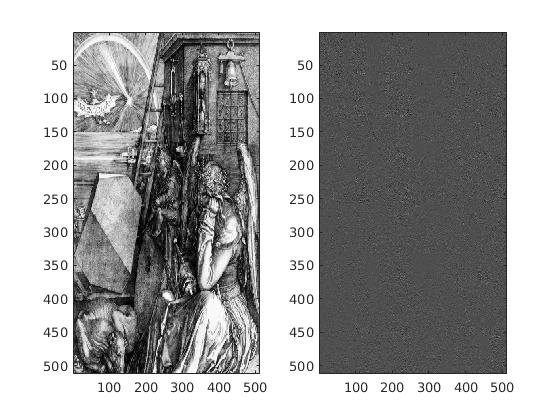
\includegraphics[scale=0.6]{Problem4_origin_vs_haar}
\medskip\\
(5)
A similar process to the one described in problem 4 was used to get the functions {\tt haar2D\_n} and {\tt haar\_inv2D\_n}.
We used {\tt haar2D\_n} to compute the normalized matrix C given by:

$$\begin{pmatrix}
682.1250 &  51.8750 &  15.2028 &  21.3900&    6.2500 &   2.7500 &   8.2500 &   8.0000\\
   77.8750   & 5.6250 &  -7.7782 &  22.0971 &  -5.2500  & -4.2500 &   1.7500 &   7.5000\\
    7.7782 & -13.7886 &  -7.7500  &  6.7500 &   0.7071 &  -5.3033 &  -1.4142 &   2.4749\\
  38.3605 &  -0.5303 &  -3.2500 &   2.0000   &-3.1820   & 1.4142  & -1.7678 &   0.3536\\
  -17.0000 &  11.5000 &   6.7175 &  -1.0607&   -4.0000  &  6.5000  & -5.0000 &  -4.5000\\
    3.5000&   -9.5000  & -2.8284 &  -2.1213&  -10.0000 &   6.0000&   -5.0000&    6.0000\\
    8.2500   & 4.7500 &  -2.8284  &  1.7678    &1.5000  & -0.5000 &  -1.0000   & 0.5000\\
   15.0000 &   4.5000 &   6.0104 &   6.0104    &3.0000  & -1.5000 &  -0.5000  &  4.0000
   \end{pmatrix}$$
   
To get matrix $C_2$, we use the command {\tt round(htransform)} on matrix $A_2$ so $$C_2 = \begin{pmatrix}
682 &   51  &   14   &  22  &    0  &    0 &     0 &     0\\
    78  &    1   &   0  &   22   &   0  &    0 &     0  &    0\\
     0  &  -14    &  0  &    1 &     0 &     0  &    0  &    0\\
    38  &   -1  &   -1 &     0  &    0  &    0  &    0  &    0\\
   -17  &   11  &    0   &   0  &    0   &   0  &    0  &    0\\
     0  &  -10  &    0  &    0 &   -10 &     0   &   0  &    0\\
     0    &  0  &    0   &   0  &    0  &    0 &     0 &     0\\
    15    &  0  &    1  &    1  &    0  &    0  &    0  &    0
\end{pmatrix}$$
(6)
Here are origin, one round, two round, three round haar transformation of the image. \\
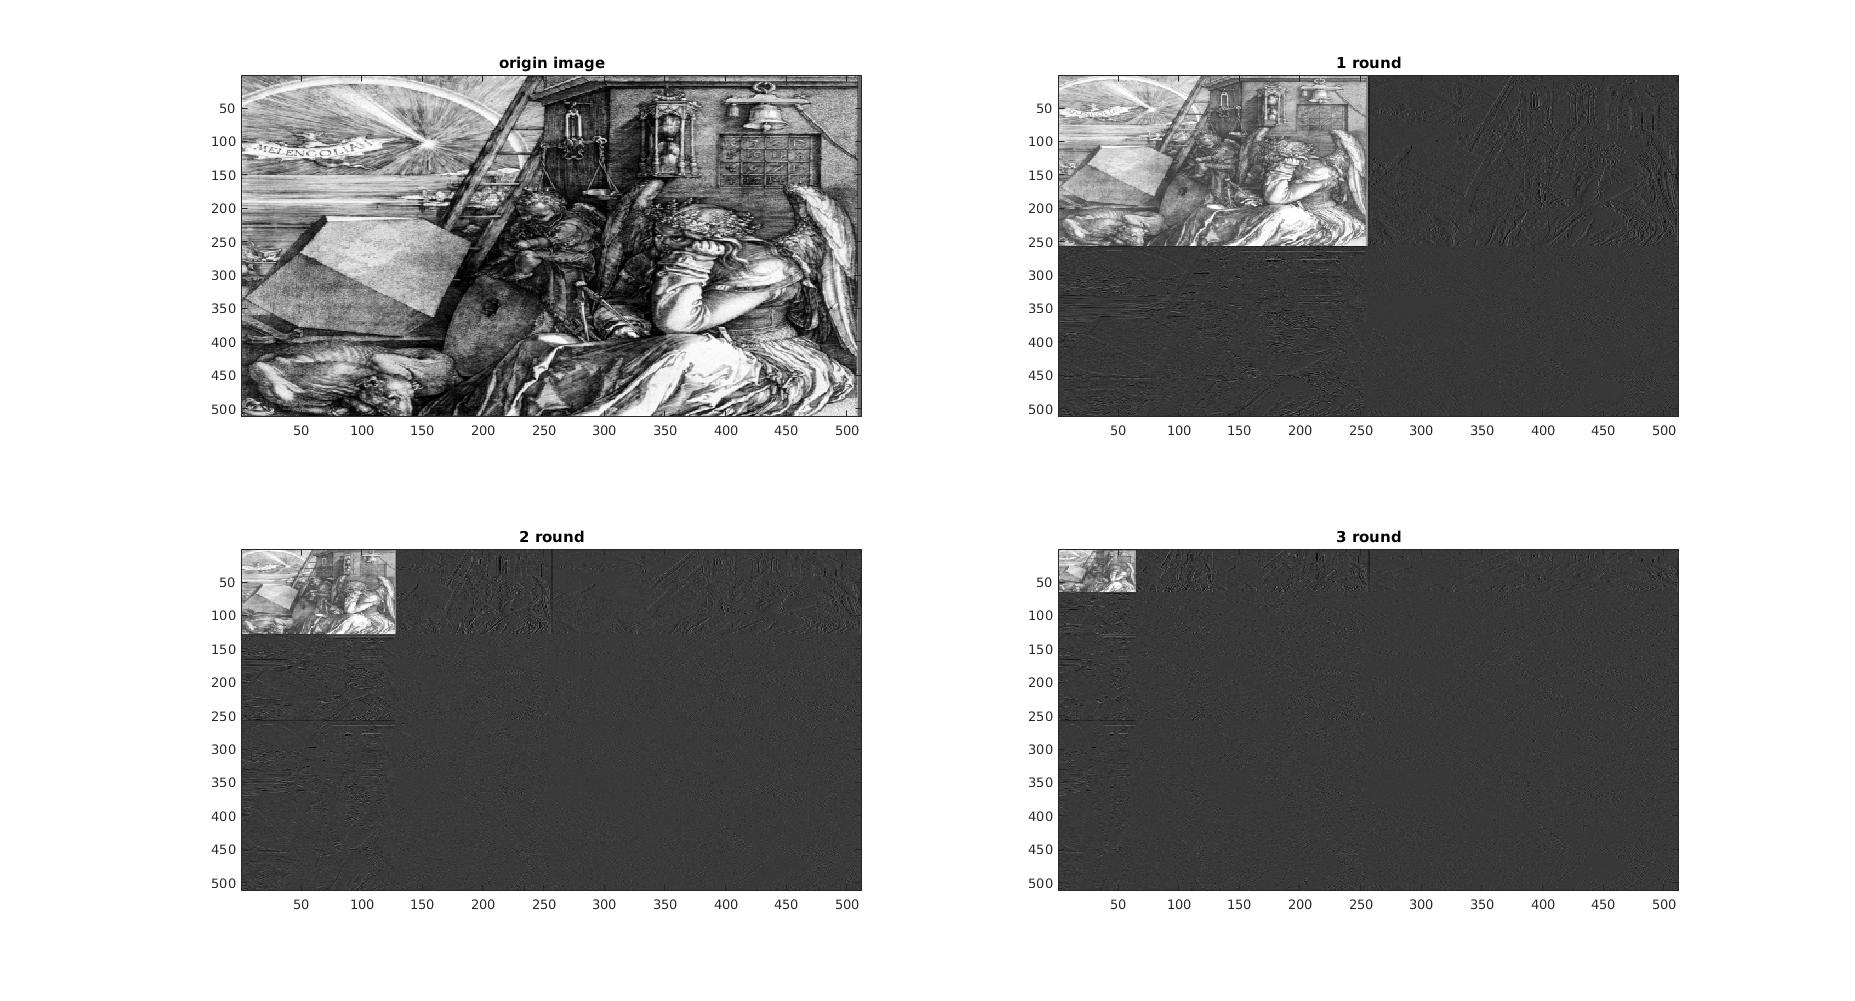
\includegraphics[scale=0.25] {Problem6_origin_vs_1_2_3_round_haar}

\end{document}
